\section{Disponibilidad de código y reproducibilidad}\label{sec:reproducibilidad}

Siguiendo los estándares de reproducibilidad computacional \cite{peng2011reproducible}, todo el código del estimador, el protocolo experimental, los módulos de inferencia estadística y las pruebas automatizadas son públicos bajo licencia PolyForm Noncommercial 1.0.0 (uso gratuito para investigación y academia; licenciamiento comercial vía \texttt{edmolinares@soulspacers.com}) en el repositorio oficial \url{https://github.com/KrissV89/sm-cfhr}. La metodología documentada en este artículo corresponde a la versión congelada \textbf{\texttt{v1.0.3}} (distribución oficial \texttt{v1.0.3-polyform}; el núcleo matemático \texttt{src/adaptive\_structured\_huber.py} permanece idéntico al de \texttt{v1.0.2} con huella SHA-256 \texttt{27a9fda4fa8b7ef0d95faf9e925e47ade9ed8f25e9ea5d97d6d7cf1c00ddde83}, mientras \texttt{v1.0.3} unifica el rollout recursivo interno de HPO con \texttt{PlantRecursiveState}). A la fecha de cierre de este manuscrito no existe un DOI de software archivado en Zenodo ni se afirma publicación externa archivada.

\begin{figure}[!htbp]
\centering
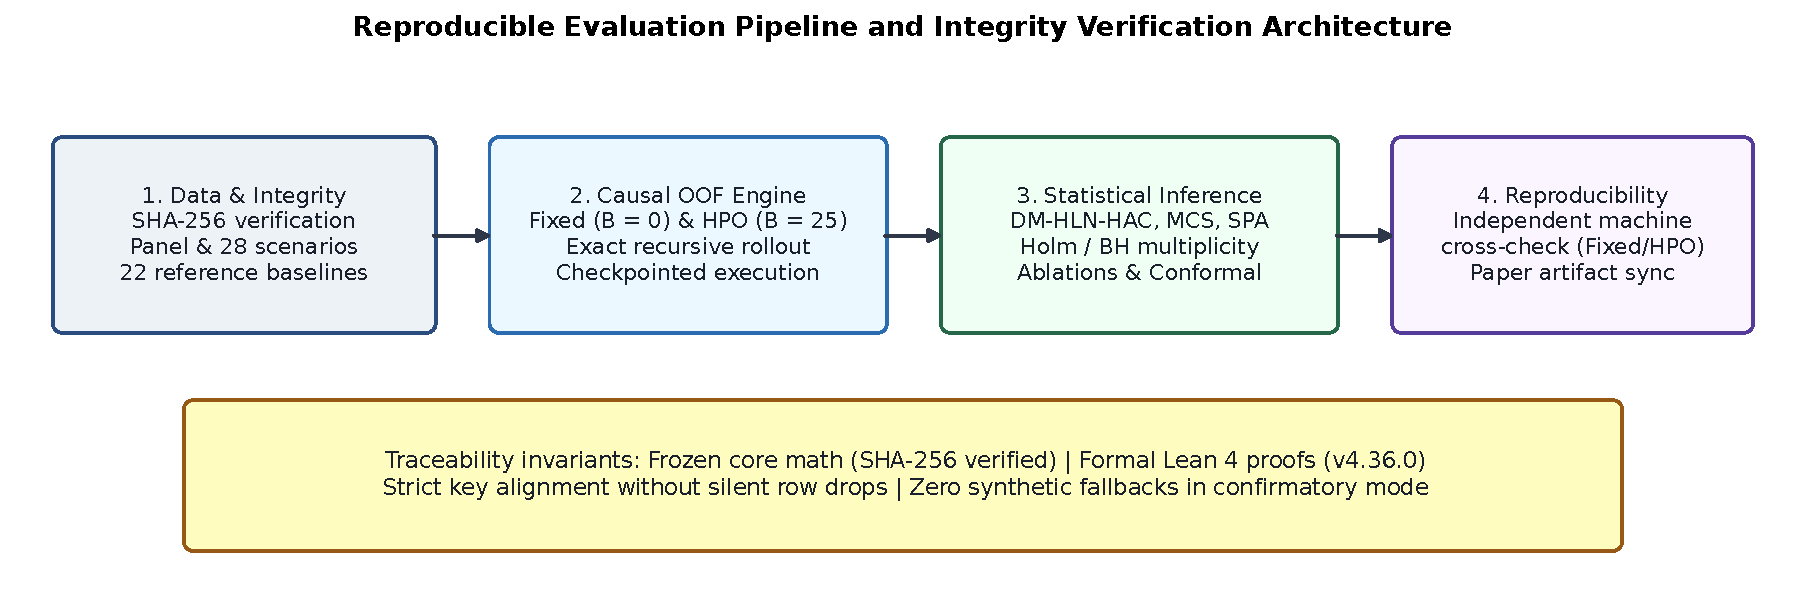
\includegraphics[width=0.98\textwidth]{figures/fig_pipeline_reproduccion.pdf}
\caption{Arquitectura de ejecución resumible, verificación de integridad mediante SHA-256 y comparación entre máquinas.}
\label{fig:pipeline_repro}
\end{figure}

El entorno computacional congelado emplea Python~$3.11.15$, NumPy~$2.3.5$, SciPy~$1.16.3$ \cite{virtanen2020scipy}, Pandas~$2.3.3$, Statsmodels~$0.14.6$, Optuna \cite{akiba2019optuna}, PyArrow y \texttt{scikit-learn}~$1.9.0$ \cite{pedregosa2011sklearn} (este último restringido a compatibilidad de API y ejecución de modelos de referencia, nunca dentro del núcleo de ajuste de SM-CFHR). Los datos originales de generación de XM y los CSV históricos de los $22$ modelos de referencia no se distribuyen en el repositorio público por restricciones de redistribución y tamaño ($603{,}70$~MB sin comprimir); para su reproducción independiente se preparó un paquete verificado de $19$ archivos CSV con manifiesto de sumas SHA-256 (\texttt{SM-CFHR-DATOS-OFICIALES-v1.0.2.zip}), importable directamente mediante el comando \texttt{python scripts/setup/import\_local\_data.py}.

La Figura~\ref{fig:pipeline_repro} resume el flujo de ejecución y auditoría disponible a través de la interfaz \texttt{python -m sm\_cfhr.cli}:
\begin{enumerate}
    \item \texttt{doctor}: verifica la integridad SHA-256 del código congelado, de los $3$ conjuntos solares principales y de los $16$ archivos de referencia que cubren los $28$ escenarios.
    \item \texttt{evaluate} / \texttt{resume}: ejecuta la evaluación OOF con persistencia granular por unidad de trabajo en fragmentos Parquet, almacenamiento SQLite para Optuna, escritura atómica (\texttt{fsync} + reemplazo atómico) y guardia de memoria RSS.
    \item \texttt{repro-bundle} y \texttt{compare-runs}: genera los siete artefactos de trazabilidad por corrida (\texttt{environment.json}, \texttt{git\_revision.json}, manifiesto de datos, configuración, ejecución y checksums) y contrasta las predicciones de dos equipos independientes bajo tolerancias relativas preespecificadas ($10^{-4}$ en Fixed y $10^{-2}$ en HPO).
\end{enumerate}
La reproducibilidad técnica (instalación limpia en entorno nuevo, verificación \texttt{doctor} y $28/28$ pruebas unitarias y anti-fuga) ha sido verificada en máquina independiente; la reproducibilidad computacional y científica de la corrida completa queda pendiente de finalizar la ejecución OOF en curso y comparar ambos equipos mediante \texttt{compare-runs}: \texttt{[PENDIENTE: RES\_COSTE\_Y\_REPRO\_INDEPENDIENTE]}.
